\documentclass{standalone}


\usepackage{tikz, pgfplots}
\usepgfplotslibrary{groupplots}
\pgfplotsset{compat=1.18} 
\usepgfplotslibrary{fillbetween}
\usepackage{adjustbox}
\begin{document}
\begin{adjustbox}{margin=4}
	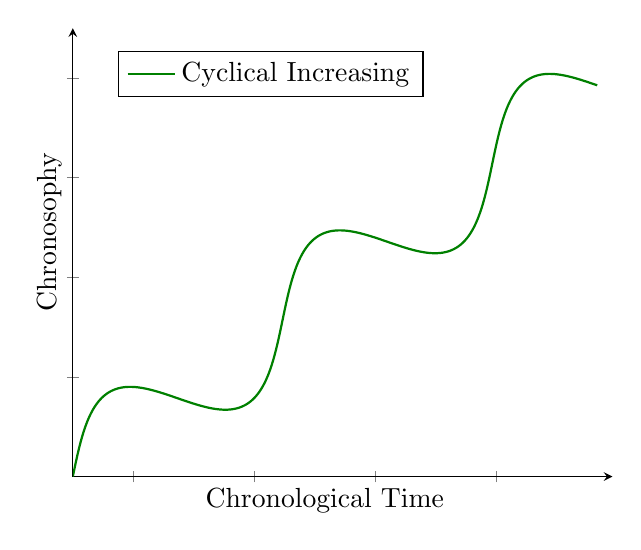
\begin{tikzpicture}		
		\begin{axis}[
			%axis y line*=left,
			%grid=both,
			%grid style={opacity=0.3},
			%xlabel=Chronological Time,
			%ylabel=Chronosophy,
			xmin = 0, xmax = 14,
			ymin=0, ymax=9,
			axis lines = center,
			xtick={0,0.5*pi,1.5*pi,2.5*pi,3.5*pi},
			ytick={2,4,6,8},
			xticklabels={\empty},
			yticklabels={\empty},
			legend style={at={(.65,0.95)}}]
			];
			
	\addlegendentry{Cyclical Increasing}
	\addplot[samples=500,color=green!50!black,smooth,thick, domain=0:5*pi]({x*(sqrt(3)/2)-sin(deg(x))*(1/2)},{x*(1/2)+sin(deg(x))*(sqrt(3)/2)});

		\end{axis}
\node[] at (3.2,-0.3) {Chronological Time};
\node[rotate=90] at (-.3,3.1) {Chronosophy};
	\end{tikzpicture}
	\end{adjustbox}
\end{document}